% last updated in April 2002 by Antje Endemann
% Based on CVPR 07 and LNCS, with modifications by DAF, AZ and elle, 2008 and AA, 2010, and CC, 2011; TT, 2014; AAS, 2016

\documentclass[runningheads]{llncs}
\usepackage{graphicx}
\usepackage{amsmath,amssymb} % define this before the line numbering.
\usepackage{algorithm}
\usepackage{algpseudocode}
\usepackage{ruler}
\usepackage{color}
\usepackage[width=122mm,left=12mm,paperwidth=146mm,height=193mm,top=12mm,paperheight=217mm]{geometry}
\begin{document}
% \renewcommand\thelinenumber{\color[rgb]{0.2,0.5,0.8}\normalfont\sffamily\scriptsize\arabic{linenumber}\color[rgb]{0,0,0}}
% \renewcommand\makeLineNumber {\hss\thelinenumber\ \hspace{6mm} \rlap{\hskip\textwidth\ \hspace{6.5mm}\thelinenumber}}
% \linenumbers
\pagestyle{headings}
\mainmatter
\def\ECCV16SubNumber{***}  % Insert your submission number here

\title{Unsupervised Deep Domain Adaptation for Pedestrian Detection} % Replace with your title

\titlerunning{ECCV-16 submission ID \ECCV16SubNumber}

\authorrunning{ECCV-16 submission ID \ECCV16SubNumber}

\author{Anonymous ECCV submission}
\institute{Paper ID \ECCV16SubNumber}


\maketitle

\begin{abstract}
This paper addresses the problem of unsupervised domain adaptation on the task of pedestrian detection in crowded scenes. First, we utilize an iterative algorithm to iteratively select and auto-annotate positive pedestrian samples with high confidence as the training samples for the target domain. Meanwhile, we also reuse negative samples from the source domain to compensate for the imbalance between the amount of positive samples and negative samples. Second, based on deep network we also design an unsupervised regularizer to mitigate influence from data noise. More specifically, we transform the last full connected layer into two sub-layers-- element-wise multiply layer and sum layer, add an unsupervised regularizer to further improve the domain adaptation accuracy. In experiments for pedestrian detection, the proposed method boosts the recall value by nearly $30\%$ while precision stays almost the same. Furthermore, we perform our method on standard domain adaptation benchmarks on both supervised and unsupervised settings and also achieve state-of-the-art results.

\keywords{Unsupervised Domain Adaptation, Unsupervised Regularizer, Deep Neural Network, People Detection}
\end{abstract}


\section{Introduction}

Deep neural network has shown great power on traditional computer vision tasks, however, the labelled dataset should be large enough to train a reliable deep model. The annotation process for the task of pedestrian detection in crowded scenes is even more resource consuming, cause we need to label concrete locations of pedestrian instances. In modern society, there are over millions of cameras deployed for surveillance. However, these surveillance situations vary in lights, background, viewpoints, camera resolutions and so on. Directly utilizing models trained on old scenes will result in poor performance on the new situations due to data distribution changes. It is also unpractical to annotate pedestrian instances for every surveillance situation.

When there are few or no labelled data in the target domain, domain adaptation helps to reduce the amount of labelled data needed. Basically, unsupervised domain adaptation aims to shift the model trained from the source domain to the target domain for which only unlabelled data are provided. Most traditional works \cite{saenko2010adapting,kulis2011you,gopalan2011domain,huang2006correcting,gretton2009covariate} either learn a shared representation between source and the target domain, or project features into a common subspace. Recently, there are also works \cite{wang2014scene,zeng2014deep,hattori2015learning} proposed to learn a scene-specific detector by deep architectures. However, heuristic methods are needed either on constructing feature space or re-weighting samples. Our motivation of developing a domain adaptation architecture is to reduce heuristic methods required during adaptation process.

In this paper, we propose a new approach for unsupervised deep domain adaptation for pedestrian detection. First, we utilize iterative algorithm to iteratively auto-annotate target examples with high confidence as positive pedestrian instances on the target domain. During each iteration, these auto-annotated data are regarded as training set to update the target model. However, these auto-annotated samples still have the limitations of lack of negative samples and existence of false positive samples, which will no doubt lead to exploration of predictions on non-pedestrian instances. Therefore, in order to compensate for the quantitative imbalance between positive and negative samples, we randomly sample negative instances from the source domain and mix into training set. Second, based on deep network, we further design an unsupervised regularizer to mitigate influence from data noise and avoid overfitting. More specifically, in order to have a better regularization effect during adaptation process, we propose to transform the last full connected layer of deep model into two sub-layers, element-wise multiply layer and sum layer. Thus, the unsupervised regularizer can be added on the element-wise multiply layer to adjust all weights in the deep network and gain better performance.

The contributions of our work are three folds.
\begin{itemize}
\item We propose an adaptation framework to learn scene-specific deep detectors for the target domains by unsupervised methodology, which adaptively select positive instances with high confidence. This can be easily deployed to various surveillance situations without any additional annotations.
\item Under this framework, we combine both supervised term and unsupervised regularizer into our loss function. The unsupervised regularizer helps to reduce influence from data noise in auto-annotated data.
\item More importantly, for better performance of unsupervised regularizer we propose to transform the last full connected layer of deep network into two sub-layers, element-wise layer and sum layer. Thus, all weights contained in the deep network can be adjusted under the unsupervised regularizer. To our knowledge, this is the first attempt to transform full connected layers for the purpose of domain adaptation.
\end{itemize}

The remainder of this paper is organized as follows. Section \ref{section:Relate Work} reviews related works. Section \ref{section:Our Approach} presents the details of our approach. Experimental results are shown in Section \ref{section:Experiment Results}. Section \ref{section:Conclusions} concludes the paper.

\section{Relate Work}
\label{section:Relate Work}

In many detection works, the generic model trained from large amount of samples on the source domain is directly utilized to detect on the target domain. They assume that samples on the target domain are subsets of the source domain. However, when the distribution of data on target and the source domain varies largely, the performance will drop significantly. Domain adaptation aims to reduce the amount of data needed for the target domain.

Many domain adaptation works try to learn a common representation space shared between source and the target domain. Saenko et al. \cite{saenko2010adapting,kulis2011you} propose a both linear-transform-based technique and kernel-transform-based technique to minimize domain changes. Gopalan et al. \cite{gopalan2011domain} project features into Grassmann manifold instead of operating on features of raw data. Alternatively, Mesnil et al. \cite{mesnil2012unsupervised} use transfer learning to obtain good representations. However, these methods have limitations since scene-specific features are not learned to boost accuracy. 

Another group of works \cite{huang2006correcting,gretton2009covariate,gong2013connecting,ghifary2014domain} on domain adaptation is to make the distribution of source and the target domain more similar. Among these works, Maximum Mean Discrepancy (MMD) is used to as a metric to reselect samples from the source domain in order to have similar distribution as target samples. In \cite{tzeng2014deep}, MMD is added on the last feature vector of the network as a regularization. Different from these methods, our work transforms the last full connected layer into two sub-layers on which MMD regularizer can be added. Thus our unsupervised regularizer can adjust all weights of the deep network during training.

There are also works on deep adaptation to construct scene-specific detector. Wang et al.\cite{wang2014scene} explore context cues to compute confidence, \cite{zeng2014deep} learn distributions of target samples and propose a cluster layer for scene-specific visual patterns. These works re-weight auto-annotated samples for their final object function and additional context cues are needed for reliable performance. However, heuristic methods are required to re-weight samples. Alternately, Hattori el al. \cite{hattori2015learning} learn scene-specific detector by generating a spatially-varying pedestrian appearance model. And Pishchulin et al. \cite{pishchulin2011learning} use 3D shape models to generate training data. However, synthesis for domain adaptation is also costly. Compared with these methods, our approach does not include the heuristic pre-processing steps. Thus, the performances of our approach are not affected by the  pre-processing steps.


\section{Our Approach}
\label{section:Our Approach}

In this section, we introduce our unsupervised domain adaptation architecture on the task of pedestrian detection in crowded scenes. Unsupervised
domain adaptation aims to shift the model trained from the source domain to the target domain for which only unlabelled data are provided. Under the unsupervised setting, we use iterative algorithm to iteratively auto-annotate target samples and update the target model. As the auto-annotated samples may contain noises, the performances may be affected by the wrongly annotated samples. Therefore, an unsupervised regularizer is introduced to mitigate the influence from data noise on the target model. Based on the assumption that the source domain and the target domain should share the same feature space after feature extraction layers, we encode an unsupervised regularizer to make a constraint that the distribution of data representation on the element-wise multiply layer should be similar between the source domain and the target domain.

The adaptation architecture of our approach consists of three parts -- the source stream, the the target stream and the unsupervised regularizer, as shown in Fig \ref{fig:streams}. The source steam takes samples from the source domain as input, while the the target stream are trained from auto-annotated positive samples from the target domain and negative samples from the source domain. These two streams can utilize any deep detection network as their basic model, as well as their detection loss function as supervised loss functions of two streams. In our experiment, we use the detection network mentioned in Section \ref{section:Detection Network} as the basic model. The unsupervised regularizer are integrated into the loss function of the the target stream.
In the following, we will first describe our iterative algorithm which iteratively selects samples from source and the target stream models, and updates the target model accordingly (\ref{Section:Iterative Algorithm}). Then, we will introduce the loss function we designed for updating the target model (\ref{Section:Loss function for the the target stream}), as well as the proposed unsupervised regularizer for improving the domain adaptation performance (\ref{section:Element-wise Multiply Layer}).


\begin{figure}
\centering
\includegraphics[height=6.5cm]{images/streams.png}
\caption{The adaptation architecture consists of three parts, the source stream, the stream and an unsupervised regularizer. The last full connected layers of both source and the target stream are transformed into element-wise layer and sum layer for the purpose of the unsupervised regularizer. Best view in colors.}
\label{fig:streams}
\end{figure}

\subsection{Iterative Algorithm}
\label{Section:Iterative Algorithm}

In this section, we introduce the iterative algorithm which is the training method of the the target stream of our adaptation architecture. There are two reasons to employ iterative algorithm. First, auto-annotated data on the target domain vary for every adaptation iteration and new positive samples will be auto-annotated as training set. Compared to methods without iterative algorithm, it helps to avoid overfitting caused by lack of data. Second, unsupervised regularizer performs better with more training data as it's a distribution based regularizer.

There are two stages for iterative algorithm. The the source stream and the the target stream are separately trained at different stages. At initialization stage, the source model of the source stream are trained under supervised loss function with abundant labelled data, (${\bf X}^{S}$,${\bf Y}^{S}$), from the source domain. After its convergence, the weights of the source model $\theta^{S}$ are taken to initialize the target stream. At adaptation stage, the target model is trained from auto-annotated positive samples (${\bf X}^{T,n}$,${\bf Y}^{T,n}$) from the target domain and randomly-selected negative samples (${\bf X}^{S,n}$,${\bf Y}^{S,n}$) from the source domain under both supervised loss function and unsupervised regularizer. Since auto-annotated data are all regarded as positive samples, negative samples from the source domain are randomly selected to compensate for lack of negative instances, which are human annotated and can thus provide true negative samples. Note that we do not jointly train two streams at adaptation stage and the weights of the source model stays static which is served as a distribution reference for unsupervised regularizer at adaptation stage. The complete adaptation process is illustrated in Algorithm \ref{algorithm:Deep domain adaptation algorithm}. After a predetermined iteration limit $N^{I}$ is reached, we obtain our final detection model on the target domain.

\begin{algorithm}
\caption{Deep domain adaptation algorithm}
\label{algorithm:Deep domain adaptation algorithm}
\begin{algorithmic}[1]
\Procedure{Deep domain adaptation} {} \\
\indent Train the source model on the source stream with abundant annotated data \\
\indent Use well-trained the source model on the source stream to initialize the target model on the target stream as $M_{0}$
\For{i = 0:$N^{I}$} \\
\indent \indent $M_{i}$ generate auto-annotated positive samples ${\bf X}^{T,n}$ of the target domain with ${\bf Y}^{T,n}$\\
\indent \indent Randomly sampled negative instances ${\bf X}^{S,n}$ from the source domain with ${\bf Y}^{S,n}$\\
\indent \indent ${\bf X}^{n} = \{{\bf X}^{T,n}, {\bf X}^{S,n}\}$ \\
\indent \indent ${\bf Y}^{n} = \{{\bf Y}^{T,n}, {\bf Y}^{S,n}\}$ \\
\indent \indent Take (${\bf X}^{n}$, ${\bf Y}^{n}$) as training data to upgrade $M_{i}$ into $M_{i+1}$
\EndFor \\
\indent $M_{N^{I}}$: final model.
\EndProcedure
\end{algorithmic}
\end{algorithm}

Different from the source domain, we use auto-annotation tools to auto-annotate pedestrian instances with high confidence as training set on the target domain. At first iteration, we take the source model as the auto-annotation tool. For subsequent adaptation iterations, updated the target model from last adaptation iteration are utilized as the auto-annotation tool. During every adaptation iteration, the auto-annotation tool (also the target model) will be updated. Thus, the training samples for the target domain at $n^{th}$ adaptation iteration may differ from that at $(n+1)^{th}$ adaptation iteration.

\subsection{Loss function for the the target stream}
\label{Section:Loss function for the the target stream}

In this section, we introduce our loss function on the the target stream of adaptation architecture, which is composed of a supervised loss and an unsupervised regularizer. The supervised loss is to learn scene-specific bias of given the target domain, while the unsupervised regularizer introduced in Section \ref{Section:Unsupervised weights regularizer on Element-wise Multiply Layer} plays an important part in reducing influence from data noise as well as avoiding overfitting.

We denote training samples from the source domain as ${\bf X}^{S} = \{x^{S}_{i}\}^{N^{S}}_{i=1}$. For training samples on the source domain, we have corresponding annotations ${\bf Y}^{S} = \{y^{S}_{i}\}^{N^{S}}_{i=1}$ with $y^{S}_{i} = (b^{S}_{i},l^{S}_{i})$, where $b^{S}_{i} = (x,y,w,h) \in R^{4}$ is the bounding box location and $l^{S}_{i} \in \{0,1\}$ is the label indicating whether $x^{S}_{i}$ is a pedestrian instance. At $n^{th}$ adaptation iteration, we have two set of training samples, auto-annotated positive samples from the target domain ${\bf X}^{T,n} = \{x^{T,n}_{j}\}^{N^{T,n}}_{j=1}$ and tantamount negative samples from the source domain ${\bf X}^{S,n} = \{x^{S,n}_{k}\}^{N^{T,n}}_{k=1}$. Their corresponding annotations can be denoted as ${\bf Y}^{T,n} = \{y^{T,n}_{j}\}^{N^{T,n}}_{j=1}$ and ${\bf Y}^{S,n} = \{y^{S,n}_{k}\}^{N^{T,n}}_{k=1}$ with $y^{T,n}_{j} = (b^{T,n}_{j},l^{T,n}_{j}\equiv1,c^{T,n}_{j})$, and $y^{S,n}_{k} = (b^{S,n}_{k},l^{S,n}_{k}\equiv0)$, respectively. $c^{T,n}_{*}$ is the confidence given by auto-annotation tools and $N^{I}$ is the maximum number of adaptation iterations. Now we can formulate the combination of supervised loss and unsupervised regularizer as follows:
\begin{eqnarray}
% \nonumber to remove numbering (before each equation)
  L(\theta^{T,n}|{\bf X}^{T,n},{\bf Y}^{T,n},{\bf X}^{S,n},{\bf Y}^{S,n},{\bf X}^{S},\theta^{S}) = L_{S} + \alpha * L_{U} \\
 \nonumber  L_{S} = \sum^{N^{T,n}}_{j=1}{H(c^{T,n}_{j})* ( R(\theta^{T,n}|x^{T,n}_{j},b^{T,n}_{j})+C(\theta^{T,n}|x^{T,n}_{j},l^{T,n}_{j}) )} \\
             + \sum^{N^{T,n}}_{k=1}{( R(\theta^{T,n}|x^{S,n}_{k},b^{S,n}_{k})+C(\theta^{T,n}|x^{S,n}_{k},l^{S,n}_{k}) )}\\
  L_{U} = L_{EWM}(\theta^{T}|{\bf X}^{T},{\bf X}^{S},\theta^{S}) \label{Eq:lmmd}
\end{eqnarray}
where $L_{S}$ is supervised loss to learn the scene-specific detector and $L_{U}$ is the unsupervised regularizer part. $H(\cdot)$ is a step function in order to select positive samples with high confidence among auto-annotated data on the target domain. $R(\cdot)$ is a regression loss for bounding box location, such as norm-1 loss, and $C(\cdot)$ is a classification loss for bounding box confidence, such as cross-entropy loss. And $L_{EWM}(\cdot)$, to be introduced in Section \ref{section:Element-wise Multiply Layer}, is the MMD-based loss added on the element-wise multiply layer for unsupervised regularization. $\alpha$ is the coefficient balancing the effect of supervised and unsupervised loss.


\subsection{Unsupervised weights regularizer on Element-wise Multiply Layer}
\label{Section:Unsupervised weights regularizer on Element-wise Multiply Layer}

As mentioned before, unsupervised regularizer plays an important role in in reducing influence from data noise and avoiding overfitting. In this paper, we propose to transform the last full connected layer in order to have better effect on unsupervised regularization.

\subsubsection{Element-wise Multiply Layer}
\label{section:Element-wise Multiply Layer}
In deep neural network, the last feature vector layer are taken as an important data representation of input images. However, in this paper, we take one step further to focus on the last full connected layer which serves as an decoder to decode rich information of the last feature vector into final outputs. As the source model is trained with abundant labelled data on the source domain, the weights of the last full connected layer are also well converged. A regularizer on the last full connected layer can adjust all weights of the network compared with that on the last feature vector layer. Denote the last feature vector, weights of the last full connected layer and final outputs as $\vec{f}_{(1\times N^{D})}$, ${\bf C}_{(N^{D}\times N^{O})}$ and $\vec{p}_{(1\times N^{O})}$. $ N^{D}, N^{O}$ are the dimension of feature vector and the dimension of output layer, respectively. Thus the operation of the full connected layer can be formulated as matrix multiply:
\begin{eqnarray}
% \nonumber to remove numbering (before each equation)
  \vec{p} &=& \vec{f}*{\bf C} \label{eq:matrixmultiply}
\end{eqnarray}
where
\begin{eqnarray}
% \nonumber to remove numbering (before each equation)
  p_{o} &=&  \sum_{d}{f_{d}*C_{d,o}}
\end{eqnarray}
Inspired by this form, we separate the above formula into two sub-operations -- element-wise multiply and sum, which can be formulated as:
\begin{eqnarray}
% \nonumber to remove numbering (before each equation)
  \vec{m}_{o} &=& [f_{d} * C_{d,o}]^{N^{D}}_{d=1} \label{eq:elementwisemultiply} \\
  p_{o} &=& \vec{m}_{o}*\vec{\overrightarrow{1}}
\end{eqnarray}
where ${\bf M}_{(N^{O}\times N^{D})} = [\vec{m}_{o}]$ is the intermediate results of element-wise multiply operations. $\vec{m}_{o}$ is a vector with $N^{D}$ dimensions, which will be the object of unsupervised regularizer. Finally, we can equivalent-transform the last full connected layer between the last feature vector layer and final outputs layer into element-wise multiply layer and sum layer. The transformed element-wise multiply layer is thus the last layer with weights before output layers. Fig \ref{fig:elementwiselayer} illustrates the transformation.

\begin{figure}
\centering
\includegraphics[height=6cm]{images/elementwiselayer.png}
\caption{Illustration of transformation of the full connected layer ${\bf C}$ into element-wise multiply layer and sum layer. After the transformation, the element-wise layer become the last layer which contains weights before output layer $\vec{p}$. Thus, an unsupervised regularizer can be added on $\vec{m_{o}}$.}
\label{fig:elementwiselayer}
\end{figure}

\subsubsection{Unsupervised regularizer on Element-wise Multiply Layer}

This section introduces our unsupervised regularizer. As stated in Section \ref{Section:Iterative Algorithm}, there are false positive samples among auto-annotated data, which will mislead the network and result in worse performance. Thus, we designed an unsupervised regularizer to mitigate the influence. We have the assumption that the dimensions of element-wise multiply layer of the last full connected layer has well converged under the training of abundant source samples. Thus, when the tasks are similar, the distribution of data representations of element-wise multiply layer on the source domain and the target domain should also be similar. When we train with false positive samples, they are easier to mutate the distribution of data representations. This observation can be illustrated in Fig \ref{fig:mmd}, where the center of $m_{o}$ of true target samples is far closer to the center of source samples, compared to that of false target samples. Confining that the distribution of data representations between source and the target domain to be similar helps to reduce the influence caused by data noise to some extent.

\begin{figure}
\centering
\includegraphics[height=4.5cm]{images/mmd.pdf}
\caption{Comparison of the center of $m_{o}$ between true and false samples on the first 20 dimensions. The center of $m_{o}$ of true target samples is far closer to the center of source samples, compared to that of false target samples. This observation supports our assumption that false instances among auto-annotated target samples tend to mutate the distribution of data representations on the element-wise multiply layer.}
\label{fig:mmd}
\end{figure}

To encode this similarity, we utilize MMD (maximum mean discrepancy)\cite{huang2006correcting} to compute distance between distributions of element-wise multiply layer of the source domain and the target domain:
\begin{equation}\label{equation:LMMD}
  L_{EWM}(\theta^{T,n}|{\bf X}^{S},{\bf X}^{T,n},\theta^{S}) = \frac{1}{N^{O}} \sum^{N^{O}}_{o=1}{ \parallel \frac{\sum^{N^{T,n}}_{j=1}{(\vec{m}^{T,n}_{o}|x^{T,n}_{j})}}{N^{T,n}} - \frac{\sum^{N^{S}}_{i=1}{(\vec{m}^{S}_{o}|x^{S}_{i})}}{N^{S}} {\parallel}^{2}  }
\end{equation}
which can also interpreted as the Euclidean distance between the center of $\vec{m}^{T,n}_{o}$ and $\vec{m}^{S}_{o}$ across all output dimensions. As a comparison, the MMD regularizer on feature vector layer can be formulated as:
\begin{equation}\label{equation:LMMD}
  L_{FV}(\theta^{T,n}|{\bf X}^{S},{\bf X}^{T,n},\theta^{S}) = \parallel \frac{\sum^{N^{T,n}}_{j=1}{(\vec{f}^{T,n}|x^{T,n}_{j})}}{N^{T,n}} - \frac{\sum^{N^{S}}_{i=1}{(\vec{f}^{S}|x^{S}_{i})}}{N^{S}} {\parallel}^{2}
\end{equation}
where $\vec{f}$ is data of the feature vector layer in Equation \ref{eq:matrixmultiply} and $\vec{m}_{o}$ is the data of the element-wise multiply layer in Equation \ref{eq:elementwisemultiply}.

Since it's unpractical to get the distribution of the whole training set, while too few images cannot obtain a stable distribution for regularization. In our experiments, the $L_{EWM}(\cdot)$ loss is calculated for every batch. An example comparison of centers of $\vec{m}^{S}_{o}$ of different batches are shown in Fig \ref{fig:mmd2}.

\begin{figure}
\centering
\includegraphics[height=4.5cm]{images/mmd2.pdf}
\caption{Comparison of the center of $\vec{m_{o}}$ between two different batches on the first 20 dimensions. These two centers are close to each other, which supports our assumption that data distributions on element-wise multiply layer between source and the target domain should be similar.  }
\label{fig:mmd2}
\end{figure}



\subsection{Detection Network}
\label{section:Detection Network}
Our generic detection model of adaptation architecture can be implemented by many deep detection models. In our experiemnt, we use the model proposed by Russel et al. \cite{stewart2015end}, which is an end to end detection network without any precomputed region proposals needed. It consists of a GoogLeNet \cite{szegedy2015going} for feature extraction and a RNN-based decoder for outputs of bounding boxes and corresponding confidences. Firstly, the GoogLeNet model encode the image into a feature map ($15\times20\times1024$) of which each 1024 dimension vector are data representation of its receptive field corresponding to a subregion of the image. Then the RNN-based layers will decode the data representation and sequentially predict 5 possible bounding boxes for each subregion by the order of their corresponding confidences. Finally, all outputs are summarized to give final detection results. However, among bounding boxes predicted as negative instances, both pedestrian and non-pedestrian instances are mixed. Therefore, we impede back-propagation of negative labels on the target domain during adaptation process.



\section{Experiment Results}
\label{section:Experiment Results}

In this section, we introduce our experiment results on both surveillance applications and the standard domain adaptation dataset. Our motivation for unsupervised domain adaptation method is easier deployment of deep detection model on surveillance situations. Thus, we firstly evaluate our approach on video surveillance. Then we employ our approach to standard domain adaptation benchmarks on both supervised and unsupervised settings to demonstrate the effectiveness of our method.

\subsection{Domain Adaptation on Crowd Dataset}

\subsubsection{Dataset and evaluation metrics}
To show the effectiveness of our domain adaptation approach for pedestrian detection, we collected a dataset\footnote{Our dataset will be made available soon.} consisting of 3 target scenes for the target domain. These three scenes contain 1308, 1213 and 331 unlabelled images. For each scene, 100 images are annotated for evaluation. Instead of labelling the whole body of a person, we labels the head of a person as bounding box during training. The motivation for labelling only pedestrian heads comes from detection of indoor pedestrian or in crowded scenes, where the body of a person may be invisible. The dataset for the source domain are Brainwash Dataset\cite{stewart2015end}. Brainwash Dataset consists of over 11917 images from 3 crowded scenes.

Our evaluation metrics for detection uses the protocol defined in PASCAL VOC \cite{everingham2015pascal}. To judge a predicted bounding box whether correctly matches a ground truth bounding box, their intersection over their union must exceed 50\%. And Multiple detections of the same ground truth bounding box are regarded as one correct prediction. For overall performance evaluation, the F1 score $F1 = 2*precision*recall/(precision+recall)$ are utilized. Higher F1 score means better performance. At the same time, the precision-recall curve are also plotted.

\subsubsection{Experimental settings}
We use deep learning framework Caffe \cite{jia2014caffe} as the adaptation architecture of our approach. During the adaptation, we set learning rate as 0.01 and momentum as 0.5. At initialization stage, GoogLeNet weights are firstly used to initialize the source model of the source stream, while parameters in RNN layers are randomly initialized from a uniform distribution. For each iteration, 100 auto-annotated images from the target domain and 100 annotated images from the source domain are alternatively used for training. The outputs of our detection network include bounding box locations and corresponding confidence, thus there are two full connected layers between the last feature vector layer and the final outputs. In our experiments, when unsupervised regularizer on the element-wise multiply layer predicting box confidence are added already, unsupervised regularizer on element-wise multiply layer predicting bounding box locations have little performance improvement. Experiments on 3 target scenes are executed separately.

\begin{figure}
\centering
\includegraphics[height=6cm]{images/pr_curve.pdf}
\caption{Precision-recall curve of 5 comparison methods on target scene 1.}
\label{fig:pr_curve}
\end{figure}

\begin{figure}
\centering
\includegraphics[height=5.5cm]{images/f1_score.pdf}
\caption{F1 score changes of 5 comparison methods during adaptation on target scene 1}
\label{fig:f1_score}
\end{figure}

\subsubsection{Comparison with different methods}
To demonstrate the effectiveness of our approach, 5 methods are compared among which method $L_{S}({\bf X}^{T,n},{\bf X}^{S,n})+L_{EWM}$ is our final approach:
\begin{description}
  \item[$L_{S}({\bf X}^{S})$] Source model only trained on the source domain.
  \item[$L_{S}({\bf X}^{T,n})$] Only auto-labeled samples on the target domain are used for training, and without any unsupervised regularizer.
  \item[$L_{S}({\bf X}^{T,n})+L_{EWM}$] Only auto-labeled samples on the target domain are used for training, with unsupervised MMD regularizer added on last element-wise multiply layer.
  \item[$L_{S}({\bf X}^{T,n},{\bf X}^{S,n})+L_{FV}$\cite{tzeng2014deep}] Both auto-labeled images from the target domain and labeled images from the source domain are alternately sampled for training, with unsupervised MMD regularizer added on last feature vector layer.
  \item[$L_{S}({\bf X}^{T,n},{\bf X}^{S,n})+L_{EWM}$] Both auto-labeled images from the target domain and labeled images from the source domain are alternately sampled for training, with unsupervised MMD regularizer added on last element-wise multiply layer.
\end{description}
Fig \ref{fig:pr_curve} plots the precision-recall curve of the above comparison methods in target scene 1. Also, the F1 score changes of every adaptation iteration are also depicted in Fig \ref{fig:f1_score}. Table \ref{table:detection results} gives concrete precision and recall value of the 5 comparison methods on three target scenes when the F1 scores are at their highest. Examples of adaptation results are shown in Fig \ref{fig:detectionresult}.

\begin{table}
\centering
\caption{Detection results of 5 compared methods on 3 target scenes} \label{table:detection results}
\begin{tabular}{l  c c c  c  c c c  c  c c c}
  \hline
  % after \\: \hline or \cline{col1-col2} \cline{col3-col4} ...
    &   \multicolumn{3}{c}{Scene 1}   & & \multicolumn{3}{c}{Scene 2} & &  \multicolumn{3}{c}{Scene 3}   \\
   \cline{2-4} \cline{6-8} \cline{10-12}
    & ~1-Pr~ & ~Re~ & ~F1~ &  & ~1-Pr~ & ~Re~ & ~F1~ &  & ~1-Pr~ & ~Re~ & ~F1~\\
  \hline
  $L_{S}({\bf X}^{S})$ & 0.101 & 0.187 & 0.309 &  & 0.015 & 0.683 & 0.807 &  & 0.035 & 0.412 & 0.577 \\
  $L_{S}({\bf X}^{T,n})$ & 0.245 & 0.408 & 0.530 &  & 0.632 & 0.905 & 0.524 &  & 0.176 & 0.778 & 0.800 \\
  $L_{S}({\bf X}^{T,n})+L_{EWM}$ & 0.284 & 0.476 & 0.572 &  & 0.012 & 0.837 & {\bf 0.906} &  & 0.078 & 0.653 & 0.764 \\
  $L_{S}({\bf X}^{T,n},{\bf X}^{S,n})+L_{FV}$\cite{tzeng2014deep} & 0.109 & 0.496 & 0.637 &  & 0.002 & 0.721 & 0.838 &  & 0.044 & 0.611 & 0.746 \\
  $L_{S}({\bf X}^{T,n},{\bf X}^{S,n})+L_{EWM}$ & 0.140 & 0.530 & {\bf 0.656} &  & 0.006 & 0.811 & 0.893 &  & 0.097 & 0.778 & {\bf 0.836} \\
  \hline
\end{tabular}
\end{table}

\subsubsection{Performance evaluation}
From the Table \ref{table:detection results}, we have the following observations:
\begin{itemize}
    \item Compared to method $L_{S}({\bf X}^{S})$, the recall values of other methods, which all utilize iterative algorithm for training, are explicitly larger. This implies the effectiveness of our iterative algorithm on boosting recall.
    \item The average F1 score of $L_{S}({\bf X}^{T,n})+L_{EWM}$ are larger than that of method $L_{S}({\bf X}^{T,n})$. Also, the average (1-precision) of $L_{S}({\bf X}^{T,n})+L_{EWM}$ is far smaller. Their difference in whether the unsupervised regularizer is added into loss function demonstrates that our unsupervised regularizer can mitigate the influence of data noise and thus boost F1 score.
    \item Compared to method $L_{S}({\bf X}^{T,n})+L_{EWM}$, the average F1 score of method $L_{S}({\bf X}^{T,n},{\bf X}^{S,n})+L_{EWM}$ is higher. This demonstrate the effectiveness of negative source samples added into the training set during adaptation process.
    \item Compared to method $L_{S}({\bf X}^{T,n},{\bf X}^{S,n})+L_{FV}$, the recall values of method $L_{S}({\bf X}^{T,n},{\bf X}^{S,n})+L_{EWM}$ are further increased. This shows that unsupervised regularizer added on the element-wise layer will provide better regularizer effect compared to that on the feature vector layer.
    \item Our final method $L_{S}({\bf X}^{T,n},{\bf X}^{S,n})+L_{EWM}$ achieves best results on target scene 1 and target scene 2. The performance on target scene 2 are rather close to the best result, which may result from large discrepancy of background between source and the target domain.
\end{itemize}

\begin{figure}
\centering
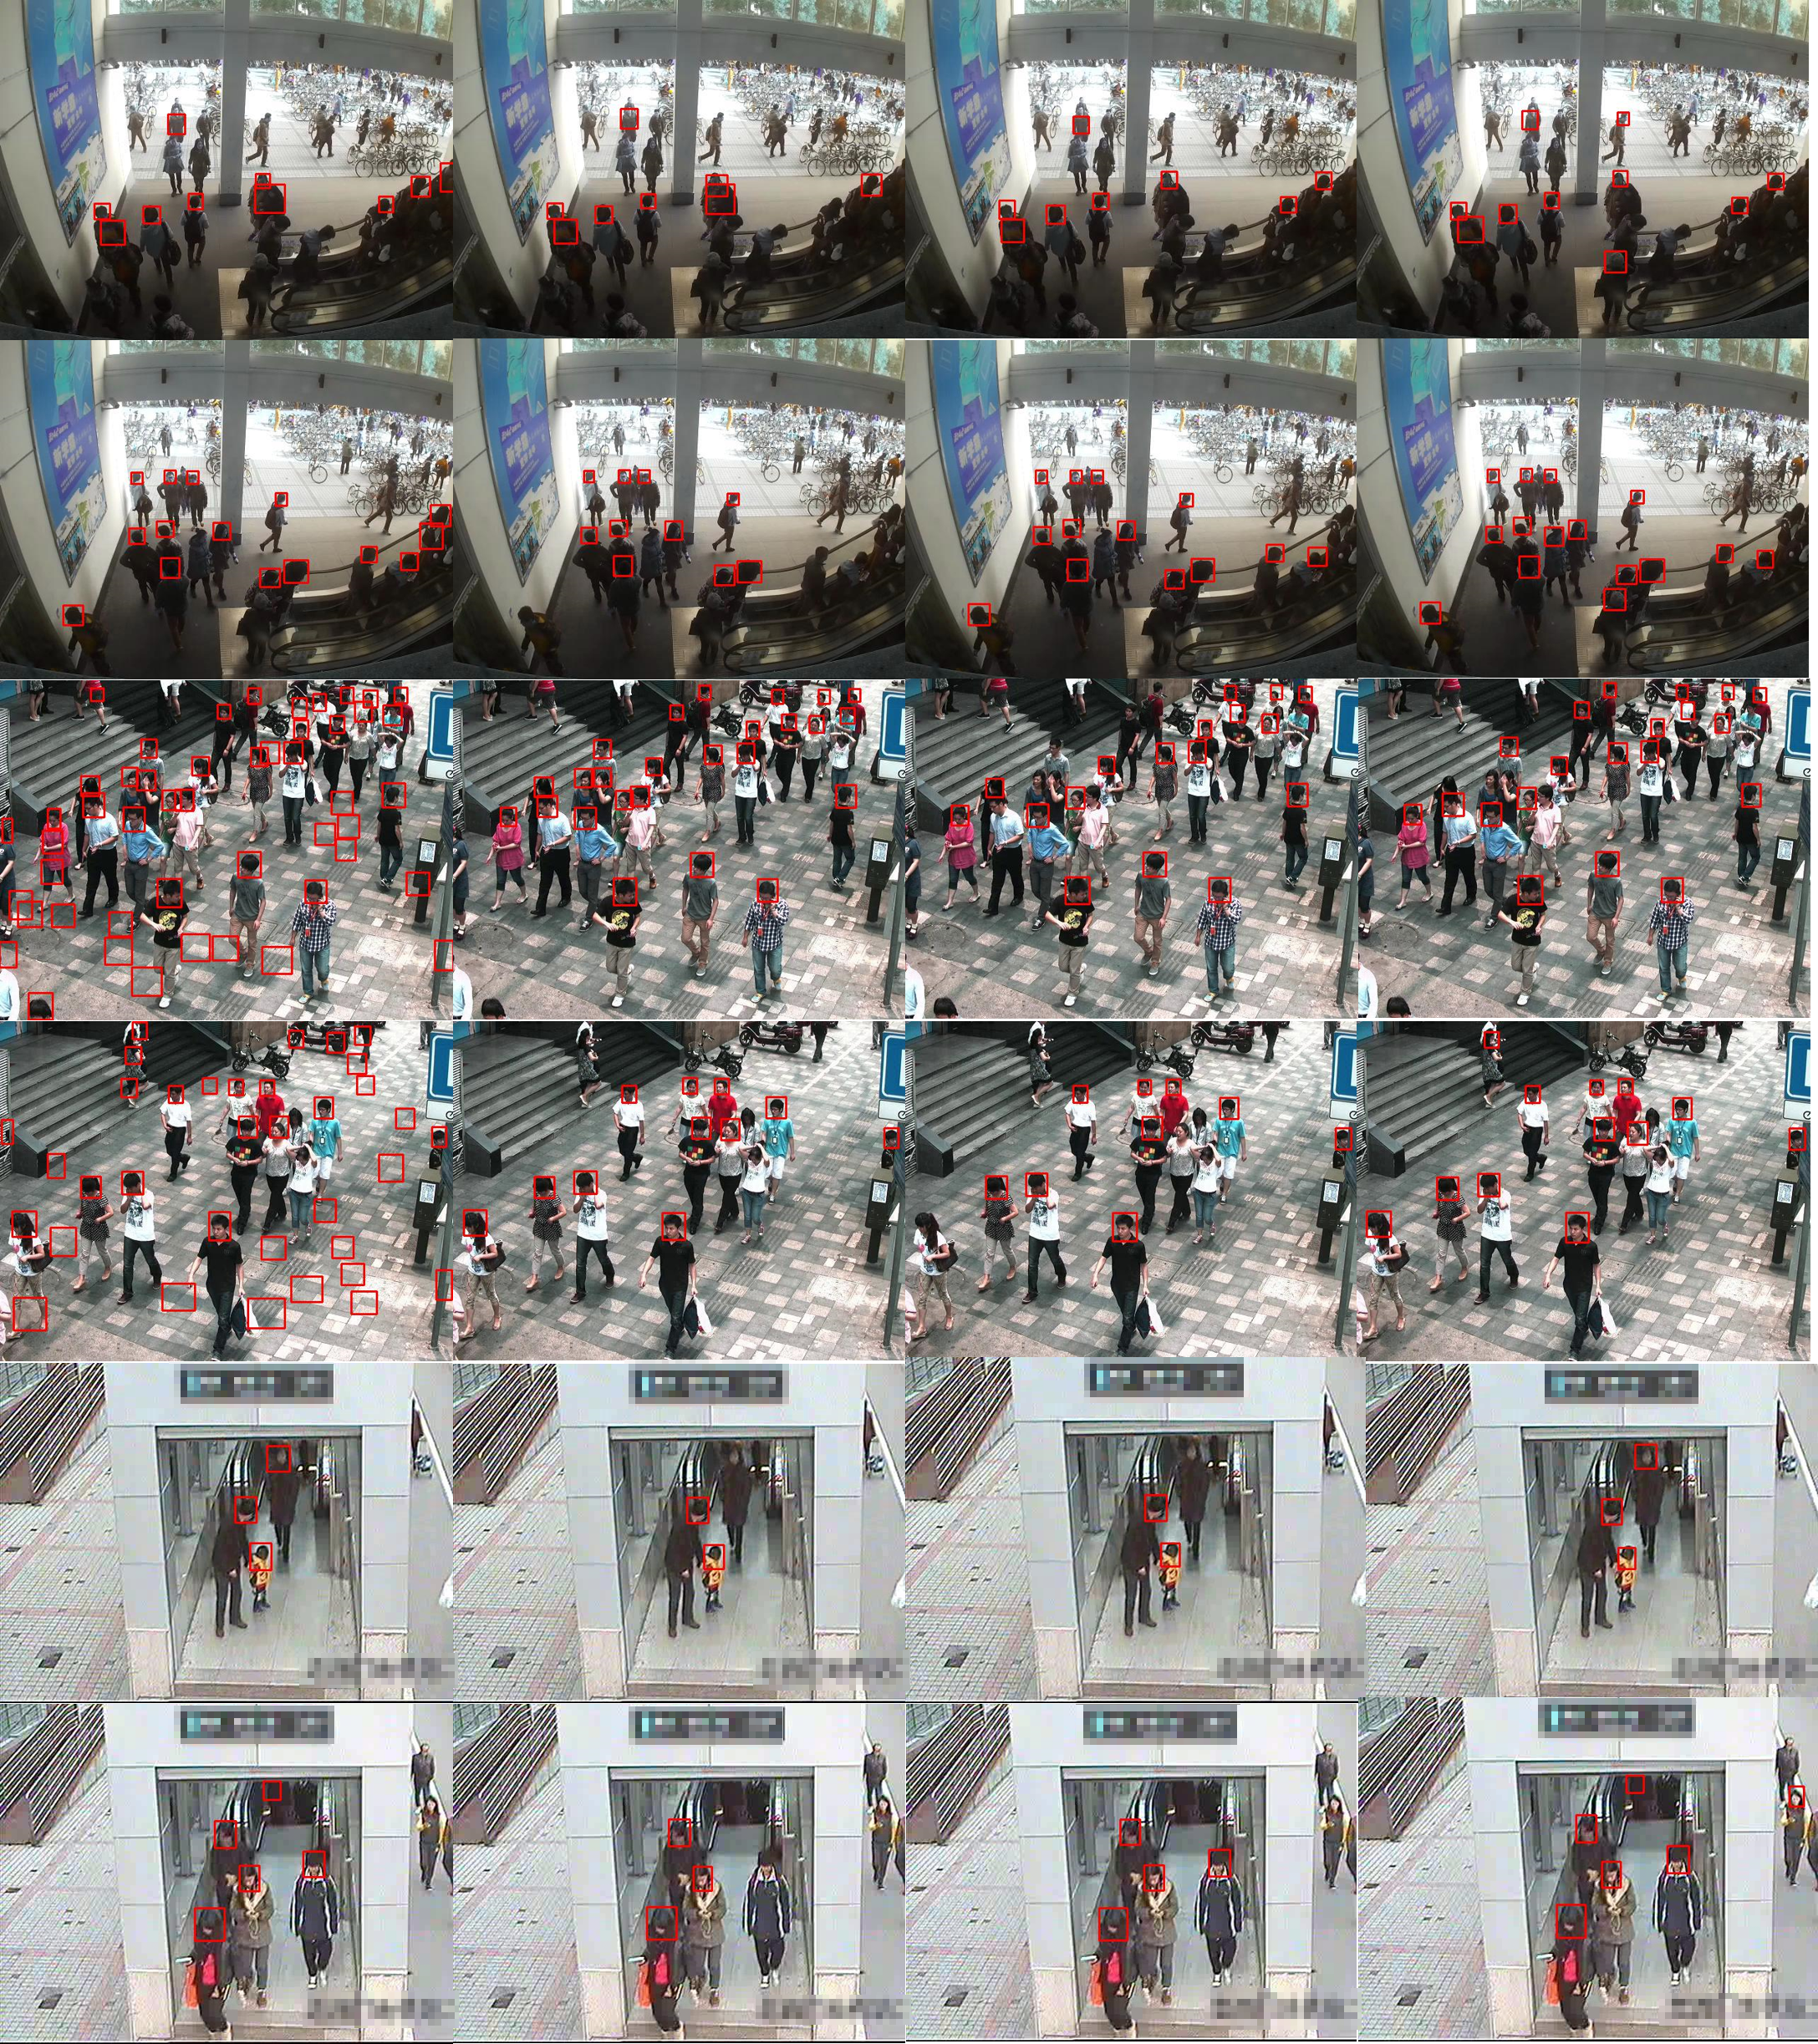
\includegraphics[height=13cm]{images/detectionresult.png}
\caption{Example results of 5 comparison methods on 3 target scenes.}
\label{fig:detectionresult}
\end{figure}


\subsection{Domain Adaptation on Standard Classification Benchmark}

In order to further demonstrate the effectiveness and generalization of our adaptation architecture, we test our method on standard domain adaptation benchmark Office dataset\cite{saenko2010adapting}.

\subsubsection{Office dataset}
The Office dataset comprises 31 categories of objects from 3 domains (Amazon, DSLR, Webcam). Example images are depicted in Fig. \ref{fig:officeimages}. As Amazon domain contains 2817 labelled images, which is the largest, we take it as the source domain and Webcam domain as the target domain. We follow the standard protocol for both supervised and unsupervised settings. Specifically, for supervised domain adaptation, we use 20 randomly sampled images with labels for each category as training data for Amazon domain. When evaluate on unsupervised domain adaptation, 3 labelled images from the target domain are additional selected for each class. For both settings, the rest of images on the target domain are used for evaluation.

\begin{figure}
\centering
\includegraphics[height=3cm]{images/officeimages.png}
\caption{Example images on Office dataset.}
\label{fig:officeimages}
\end{figure}

\subsubsection{Experimental settings and network design}
On supervised setting, we reused the architecture in pedestrian detection. We utilize AlexNet \cite{krizhevsky2012imagenet} as the generic model of both streams. Firstly, we train the source model on the source stream with provided training data from Amazon domain. Then iterative algorithm mentioned in Sec \ref{Section:Iterative Algorithm} are utilized for adaptation. The difference is, besides auto-labelled images on the target domain 3 human labelled images for each class are also included as training data for the target model. For each iteration, 100 images are randomly sampled from training data. The unsupervised MMD regularizer is added on the element-wise multiply layer transformed from the last full connect layer of the target model. We set the coefficient value $\alpha$ as 0.05 on Eq \ref{Eq:lmmd}.

We use the same experimental setting for our unsupervised adaptation, except that at adaptation stage, no human labelled images can be added into the training set.
\subsubsection{Performance evaluation}
In Table \ref{table:office}, we compare our approach with other seven recently published works in both supervised and unsupervised settings. The outstanding performance on both settings confirms the effectiveness of our iterative algorithm and MMD regularizer on the element-wise multiply layer transformed from the last full connect layer.


\begin{table}
\centering
\caption{Multi-class accuracy evaluation on Office dataset with supervised and unsupervised settings.} \label{table:office}
\begin{tabular}{l c c}
  \hline
  % after \\: \hline or \cline{col1-col2} \cline{col3-col4} ...
   & \multicolumn{2}{c}{A $\rightarrow$ W}    \\
   \cline{2-3}
   ~~~~~~~~~~~~~~~~~~~~~~~~~~~~~~~
   ~~~~~~~~~~~~~~~~~~~~~~~~~~~~~~~
    & ~Supervised~ & ~Unsupervised~ \\
  \hline
  GFK(PLS,PCA)\cite{gong2012geodesic} & 46.4 & 15.0 \\
  SA \cite{fernando2013unsupervised} & 45.0 & 15.3 \\
  DA-NBNN \cite{tommasi2013frustratingly} & 52.8 & 23.3 \\
  DLID \cite{chopra2013dlid}& 51.9 & 26.1 \\
  DeCAF${}_{6}$S \cite{donahue2013decaf} & 80.7 & 52.2 \\
  DaNN \cite{ghifary2014domain}& 53.6 & 35.0 \\
  DDC\cite{tzeng2014deep} & 84.1 & 59.4 \\
  \hline
  Ours & {\bf 85.4} & {\bf 69.3} \\
  \hline
\end{tabular}
\end{table}


\section{Conclusions}
\label{section:Conclusions}

In this paper, we introduce an adaptation architecture to learn scene-specific deep detectors for the target domains. Firstly, iterative algorithm is utilized to iteratively auto-annotate target samples and update the target model. As auto-annotated data are lack of negative samples and contain data noise, we randomly sample negative instances from the source domain. At the same time, an unsupervised regularizer is also designed to mitigate influence from data noise. More importantly, we propose to transform the last full connected layer for better regularizer effect.

Experiments on both surveillance situations and standard domain adaptation benchmarks show the effectiveness of our architecture.


\bibliographystyle{splncs}
\bibliography{egbib}
\end{document}
